\documentclass{beamer}
\usepackage{amsfonts,amsmath,oldgerm}

\usetheme{sintef}

\newcommand{\testcolor}[1]{\colorbox{#1}{\textcolor{#1}{test}}~\texttt{#1}}

\usefonttheme[onlymath]{serif}

\titlebackground*{images/default}

\newcommand{\hrefcol}[2]{\textcolor{cyan}{\href{#1}{#2}}}

\title{How reliable are Sentinel-2 cloud detection algorithms?}
\subtitle{Global uncertainty estimation with gaussian processes.}
\author{\href{mailto:csaybar@gmail.com}{Cesar Aybar}}
%\date{Written on June 6, 2016}

\begin{document}
\maketitle


\begin{chapter}[images/default]{sintefred}{Context}
\begin{itemize}
\item Available cloud datasets
\item Shortcomings
\end{itemize}
\end{chapter}


\begin{frame}{Available cloud datasets}
\begin{columns}
	\begin{column}{0.5\textwidth}
		\begin{figure}
			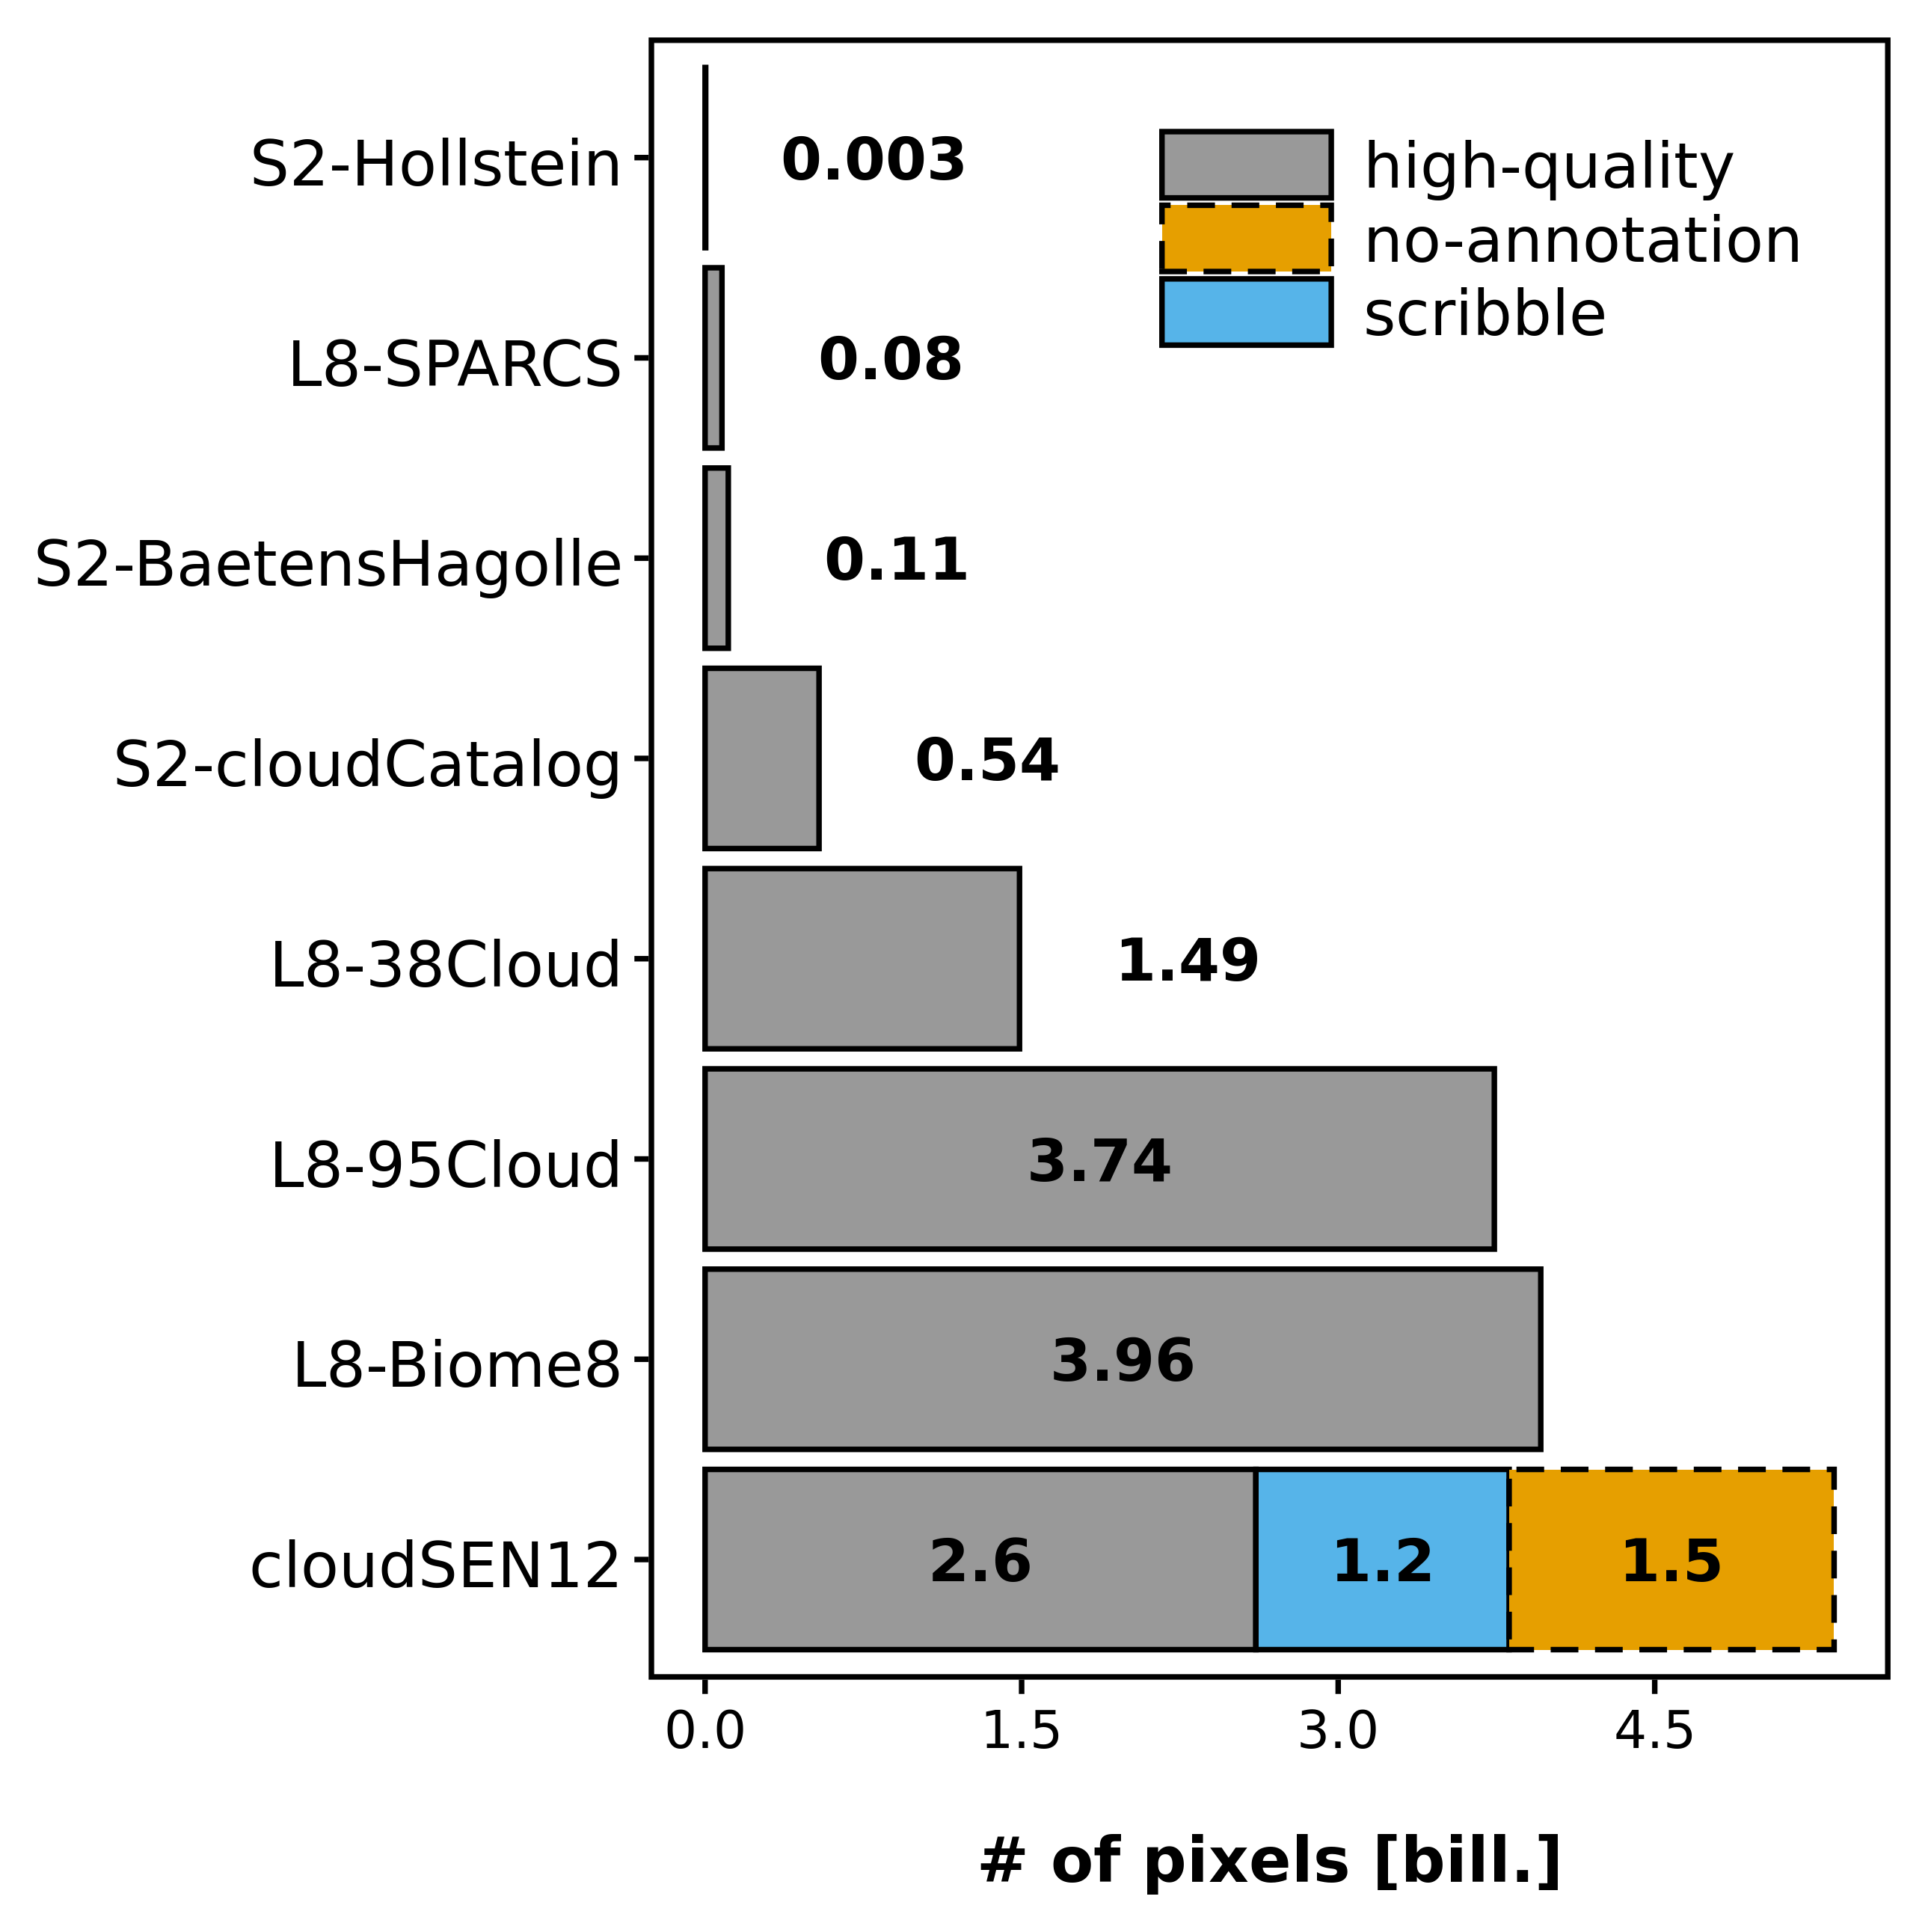
\includegraphics[width=\textwidth]{images/figure01}
		\end{figure}	
	\end{column}
	\begin{column}{0.5\textwidth}
	\begin{itemize}[<+->]
		\item Cloud labels created by human photo-interpretation.
		\item There are just three cloud shadow providers: Hollstein, SPARCS, and \textbf{cloudSEN12}.
	\end{itemize}
	\end{column}
\end{columns}
\end{frame}

\begin{frame}{Available cloud datasets}
\begin{figure}
	\centering
	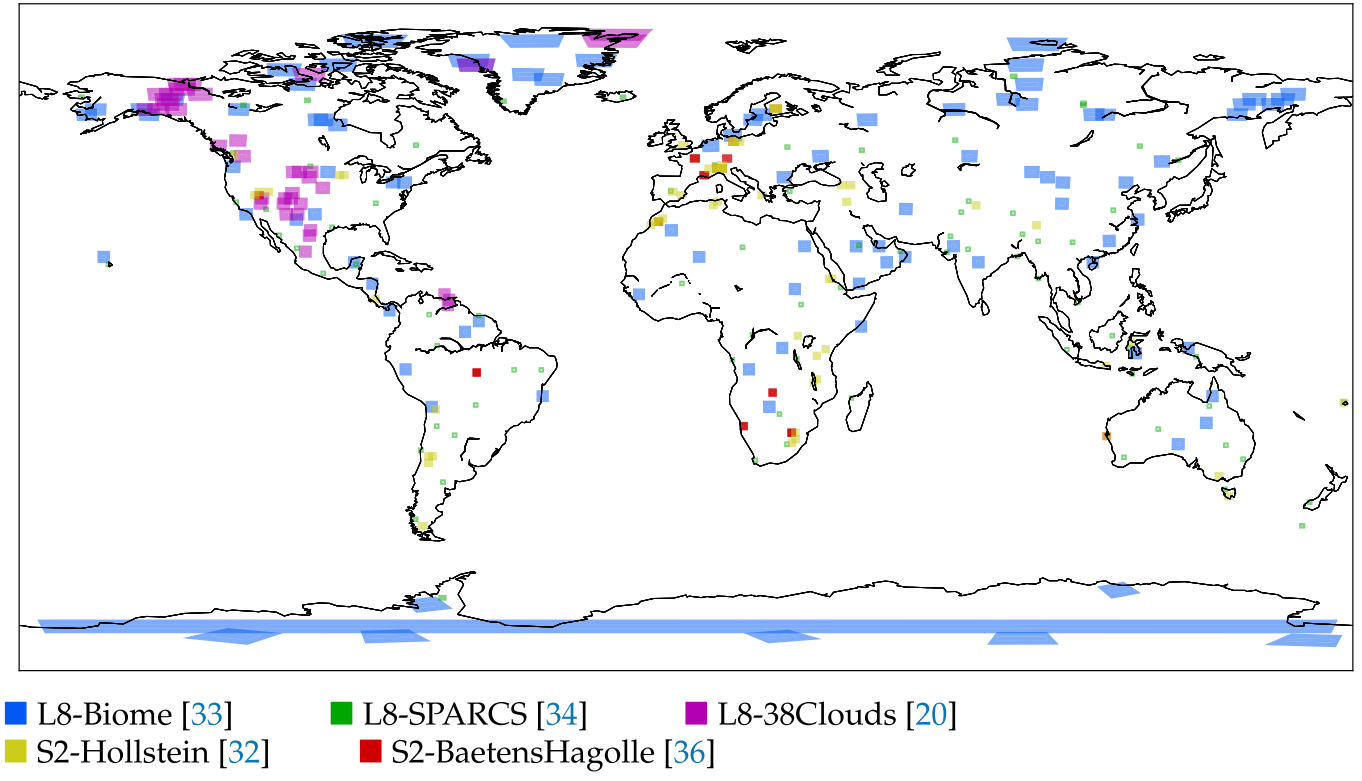
\includegraphics[width=0.75\linewidth]{images/figure_02}
\end{figure}
\end{frame}


\begin{frame}{Shortcomings}
\begin{itemize}
	\item None of them have a \textbf{time dimension}.
	\item \textbf{Downloading is a struggle}. Using STAC is a no-brainer :).
	\item As is often with EO datasets, no information regarding the \textbf{control quality} is provided.
	\item \textbf{Human level performance} is not evaluated.		
	\item High class imbalance.
	\item Geographically biased.
	\item The creation procedure is unclear.	
\end{itemize}
\end{frame}



\begin{frame}{Shortcomings}
\begin{figure}
	\centering
	
\includegraphics[width=0.65\linewidth]{images/figure04}
	\label{fig:figure04}
\end{figure}
\end{frame}


\begin{chapter}[images/default]{sintefyellow}{cloudSEN12}
	\begin{itemize}
		\item Data Preparation
		\item Image Patch Selection
		\item Labeling
	\end{itemize}
\end{chapter}

\begin{frame}{Data Preparation}
\begin{figure}
	\centering
	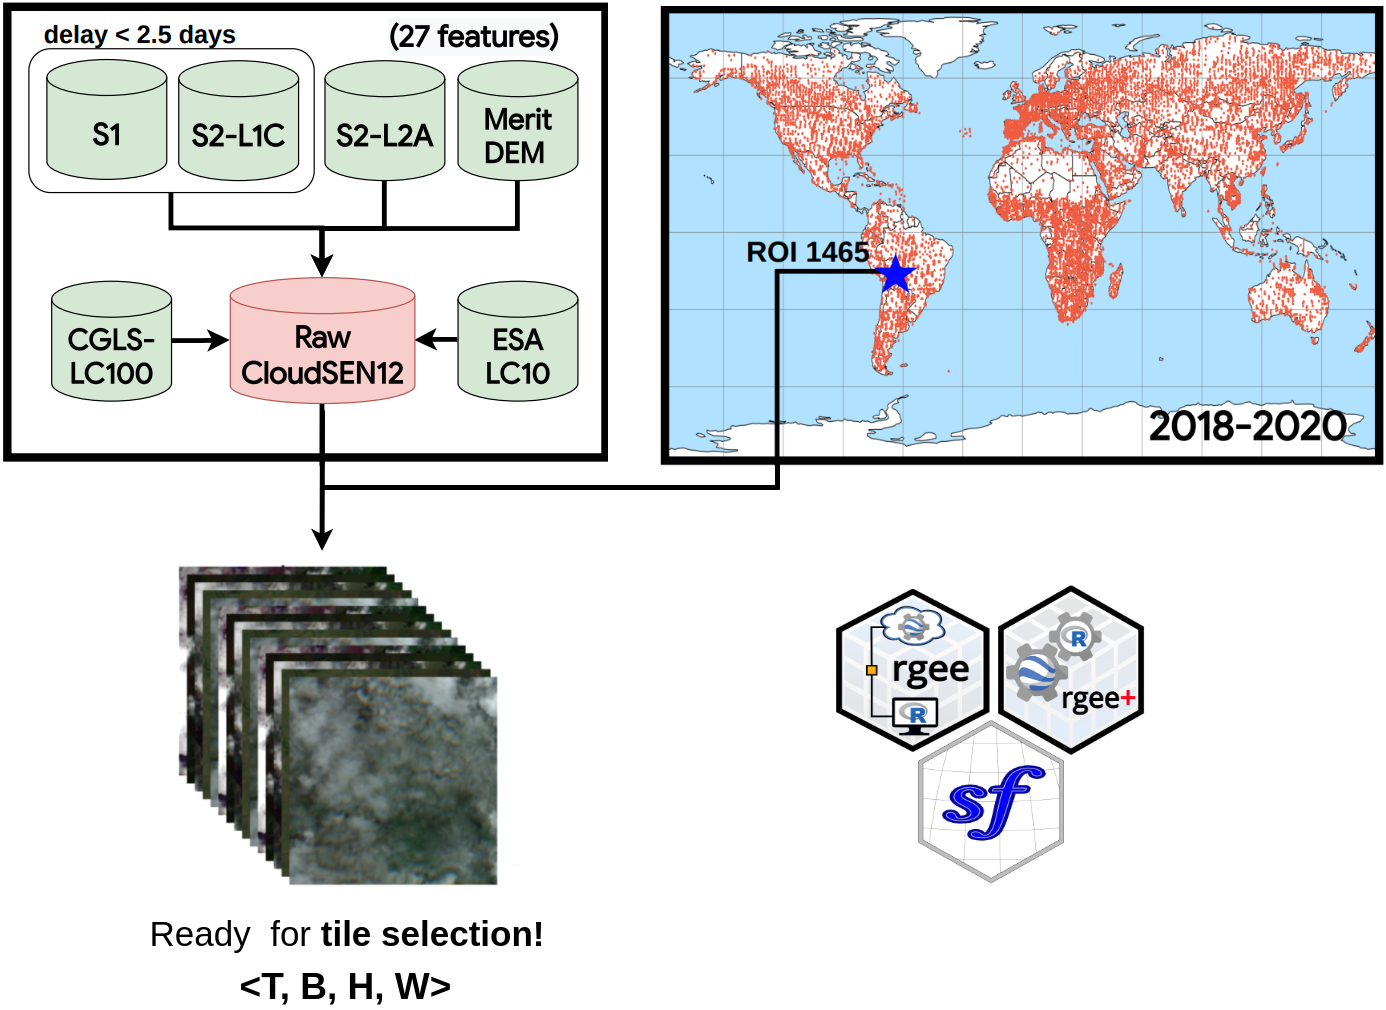
\includegraphics[width=0.7\linewidth]{images/figure_04}
	\label{fig:figure04}
\end{figure}
\end{frame}


\begin{frame}{Image Patch Selection}
	\begin{figure}
		\centering
		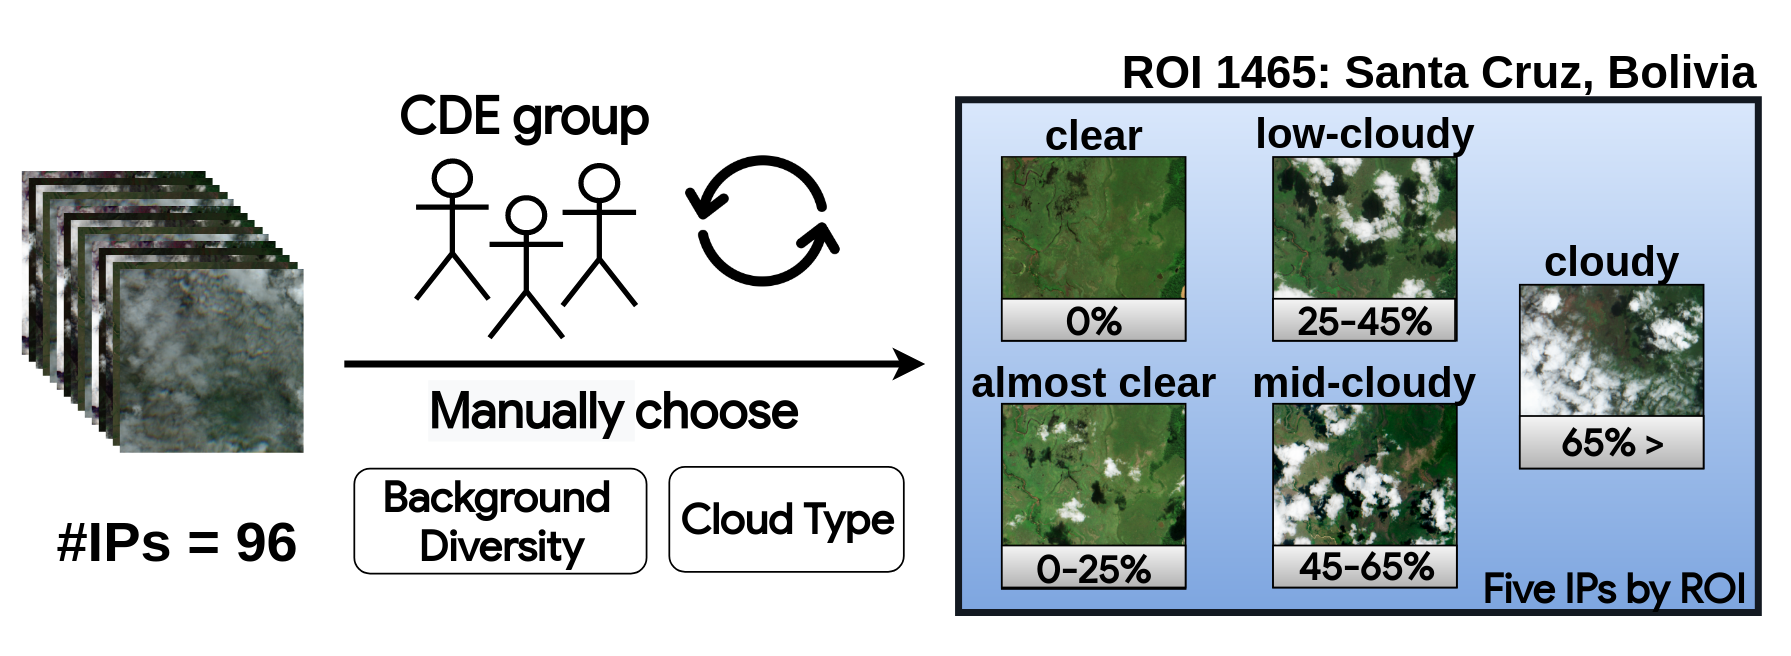
\includegraphics[width=0.9\linewidth]{images/figure_05.png}
	\end{figure}
\end{frame}


\begin{frame}{Labeling}
	\begin{figure}
		\centering
		\includegraphics[width=0.65\linewidth]{images/figure_06}
		\label{fig:figure04}
	\end{figure}
\end{frame}

\begin{frame}{Labeling}
\begin{columns}
	\begin{column}{0.5\textwidth}
		\begin{figure}
		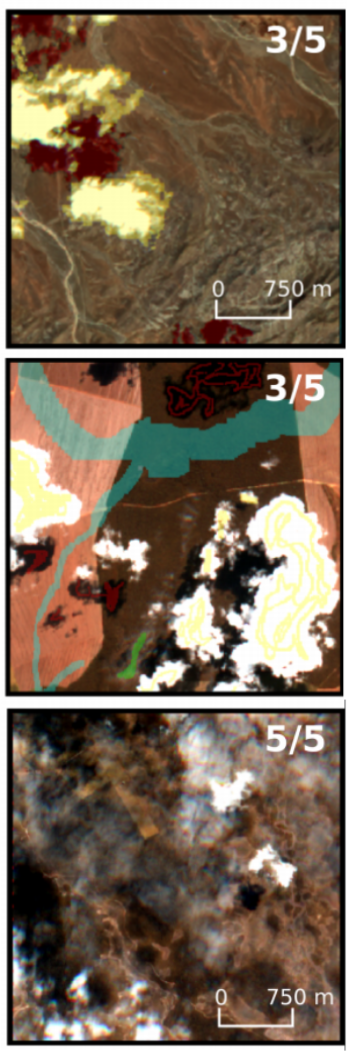
\includegraphics[width=0.32\textwidth]{images/figure_07}
		\end{figure}	
	\end{column}
	\begin{column}{0.5\textwidth}
		\begin{itemize}[<+->]
			\item \textbf{2000 ROIs} with pixel level annotation, where the average annotation time is 150 minutes (high-quality group).
			\item \textbf{2000 ROIs} with scribble level annotation.
			\item \textbf{5880 ROIs} with annotation only in the cloud-free (0\%) image (no annotation group).
		\end{itemize}
	\end{column}
\end{columns}	
\end{frame}



\begin{frame}{Data Preparation}
	\begin{figure}
		\centering
		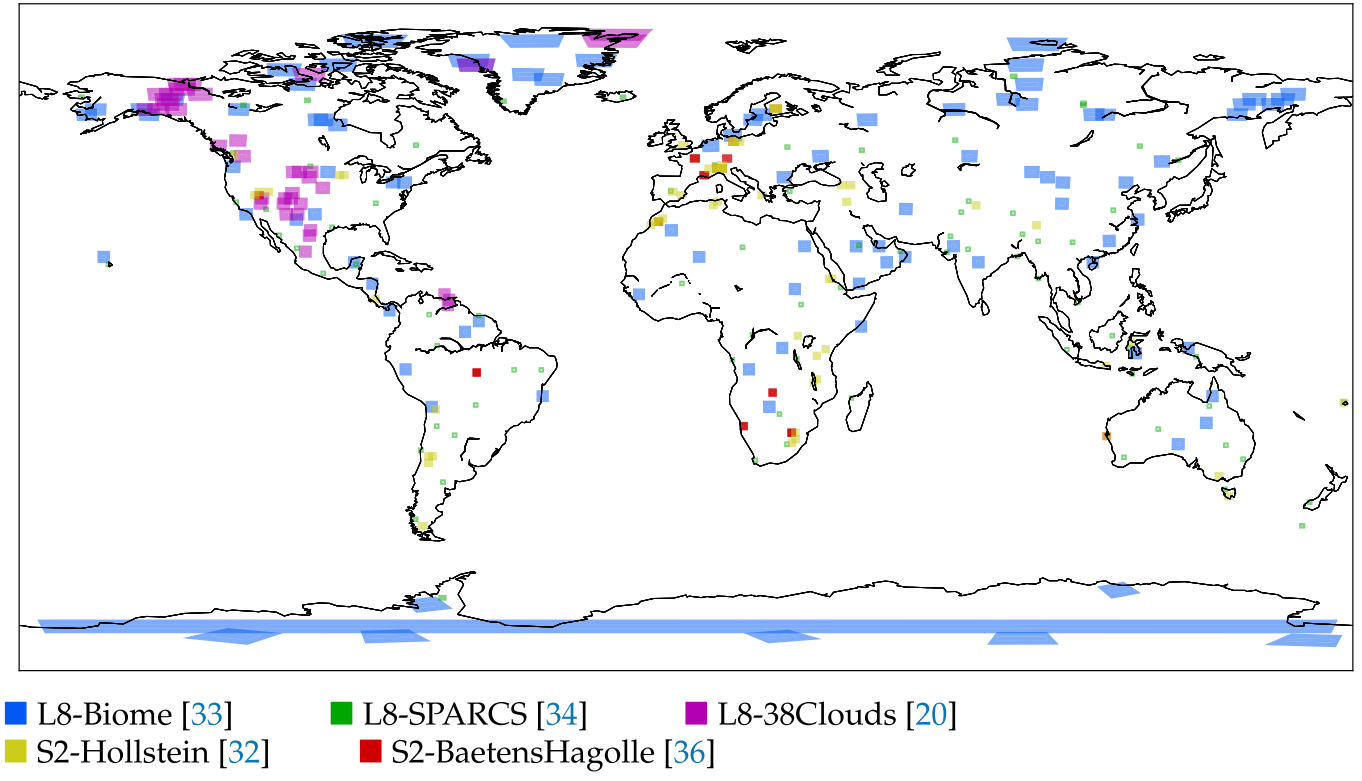
\includegraphics[width=0.75\linewidth]{images/figure_02}
	\end{figure}
\end{frame}

\begin{frame}{Data Preparation}
	\begin{figure}
		\centering
		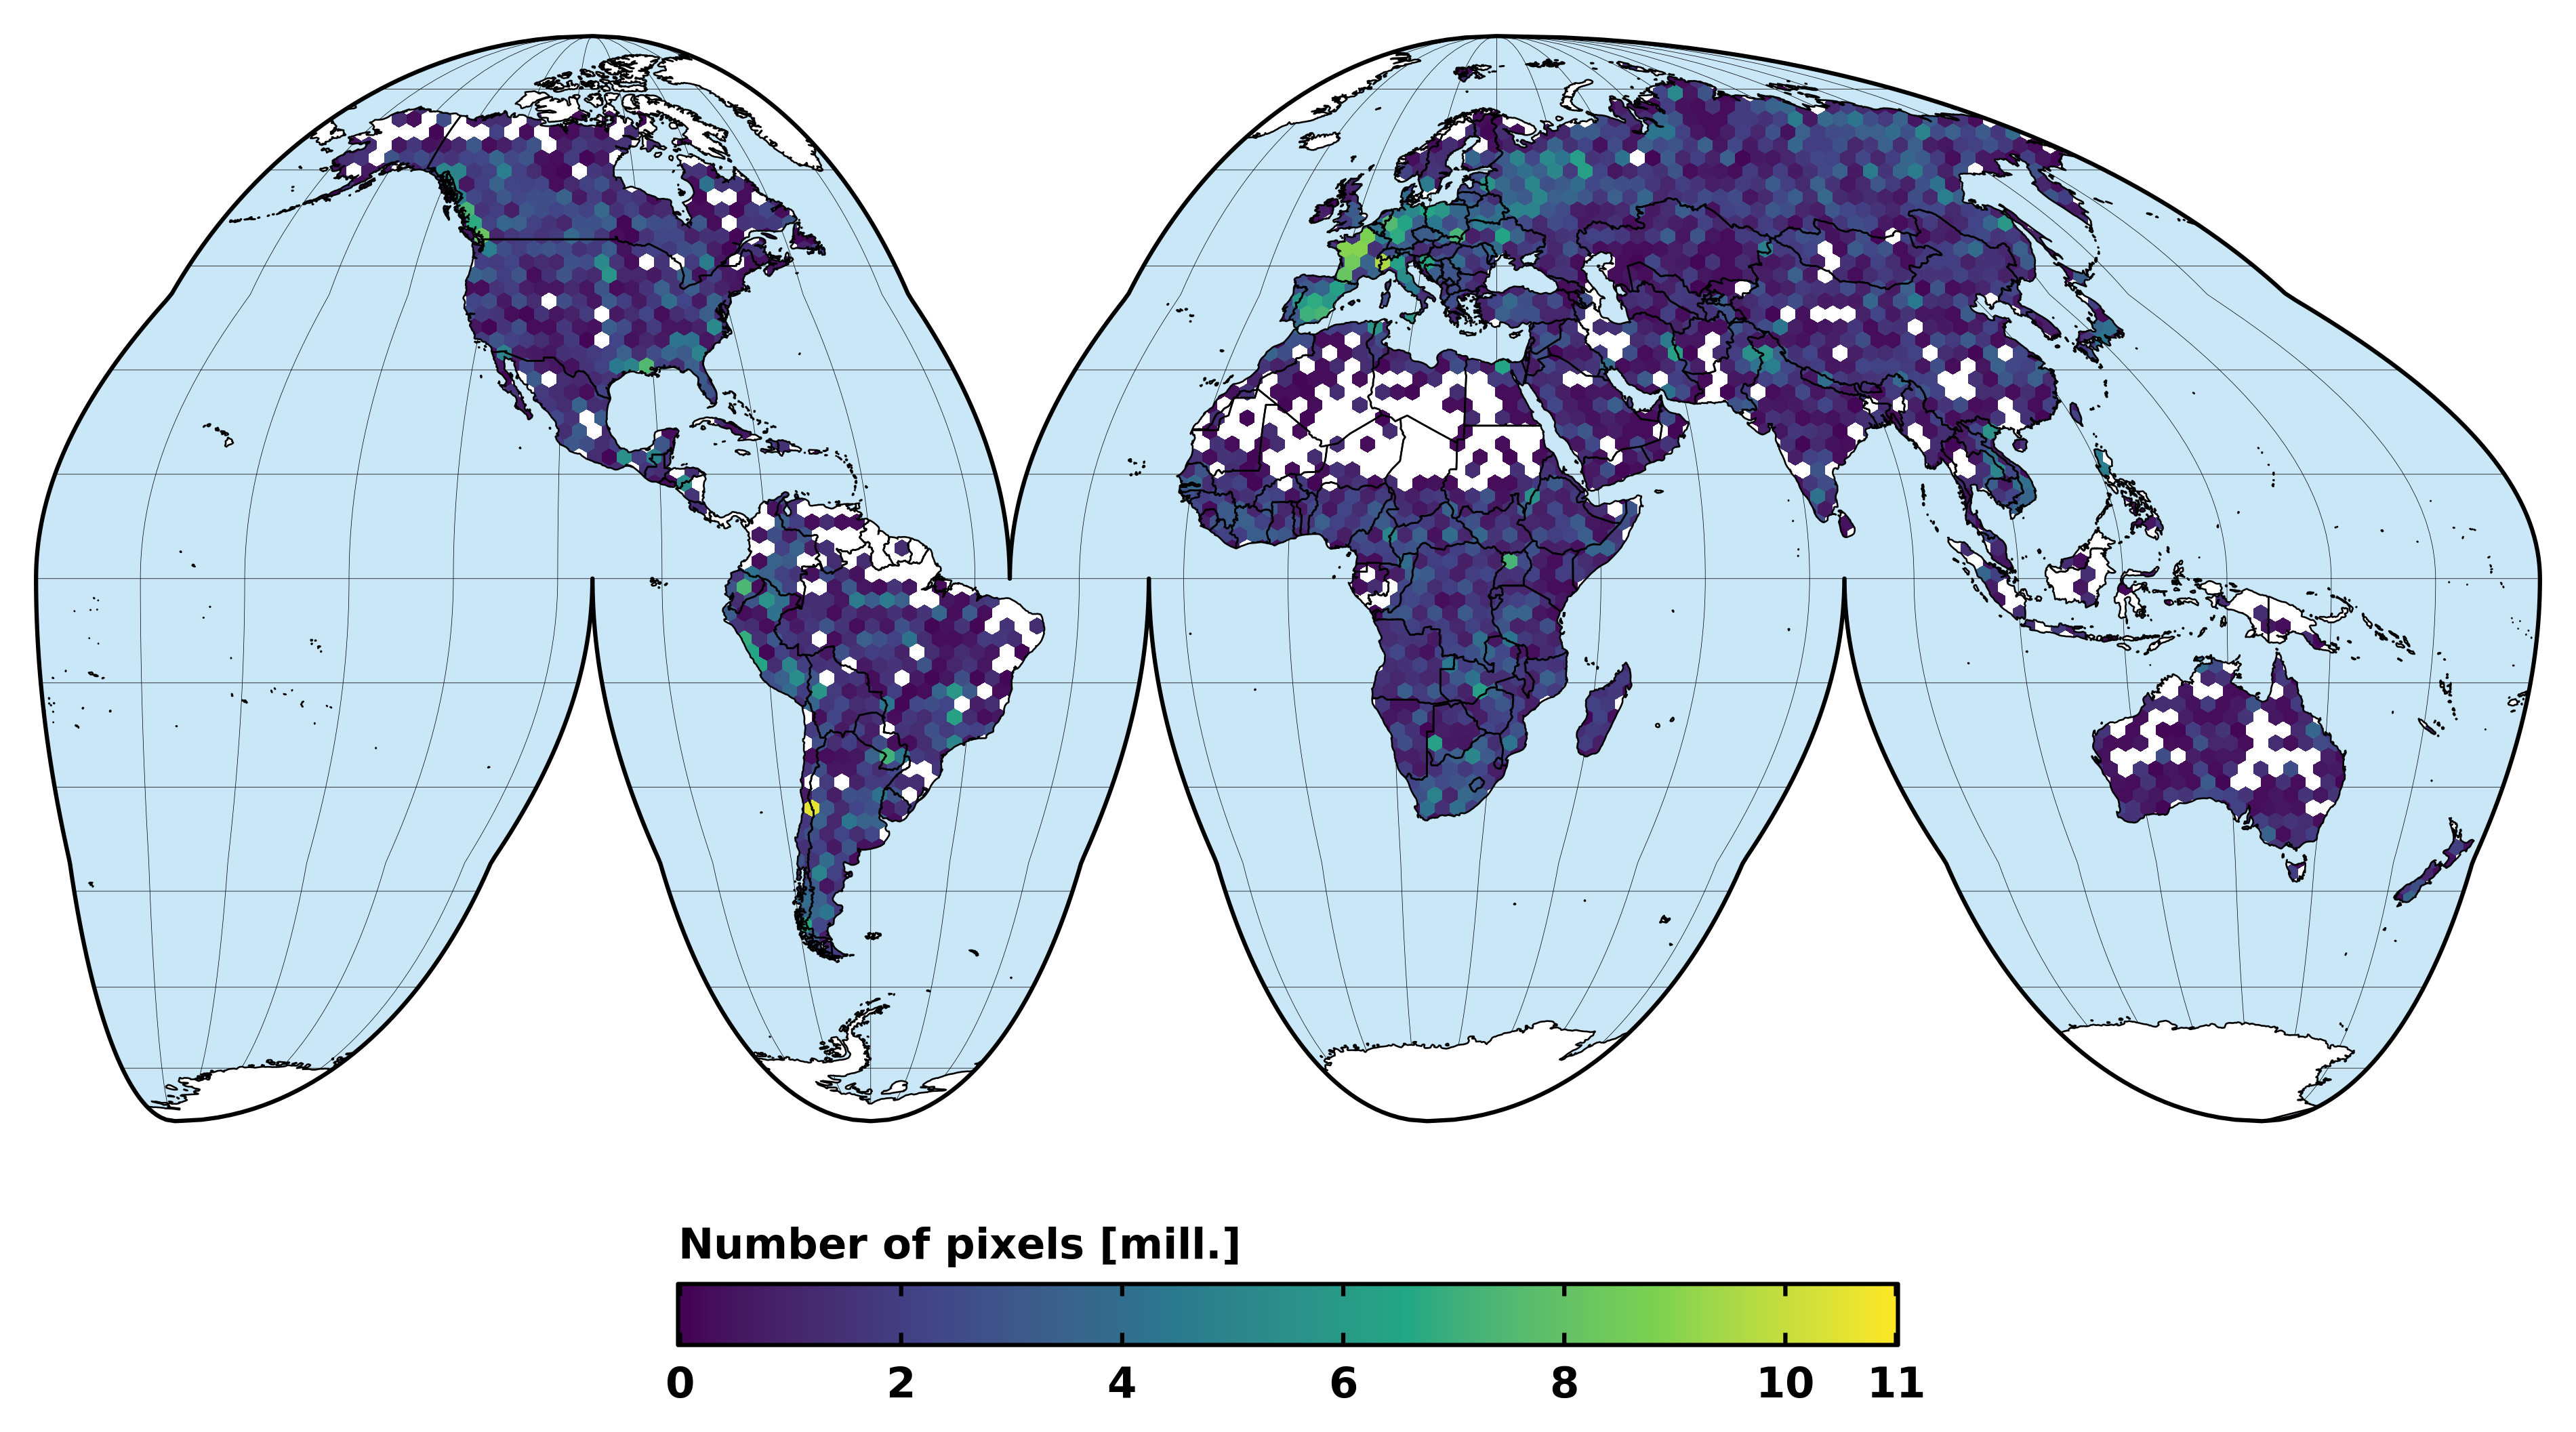
\includegraphics[width=0.85\linewidth]{images/figure_03}
	\end{figure}
\end{frame}


\begin{frame}{The website}
	\begin{figure}
		\centering
		
\includegraphics[width=0.45\linewidth]{images/logo_full.png}
	\end{figure}
	\centering
	\textbf{\hrefcol{https://cloudsen12.github.io/}{https://cloudsen12.github.io/}}
\end{frame}

\begin{chapter}[images/default]{sintefgreen}{Uncertainty estimation}
	\begin{itemize}
		\item The problem.
		\item Gaussian proccess
		\item Locally Weighted Gaussian Process
		\item 3D-kernel
		\item TODO
	\end{itemize}
\end{chapter}

\begin{frame}{The problem}
	\begin{figure}
		\centering
		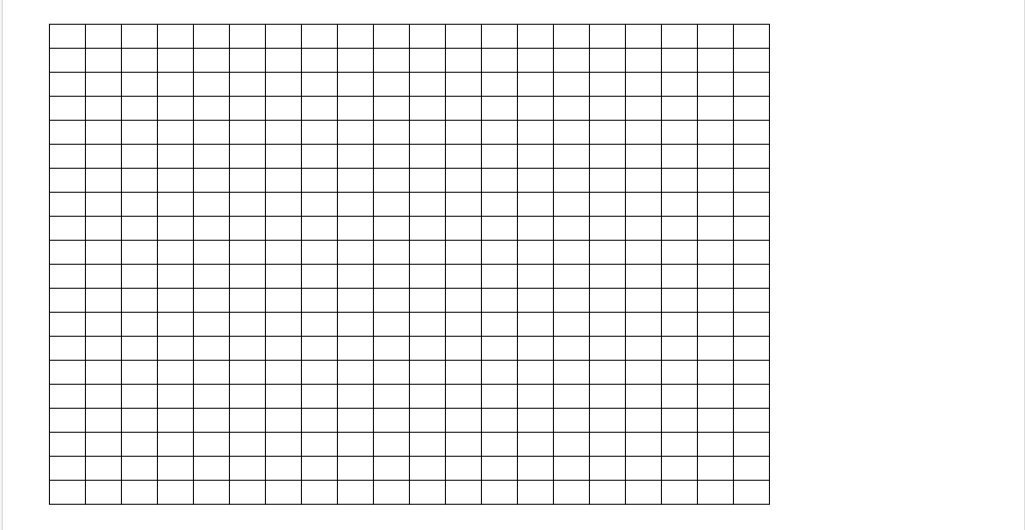
\includegraphics[width=0.85\linewidth]{images/figure_08}
	\end{figure}
\end{frame}

\begin{frame}{The problem}
	\begin{figure}
		\centering
		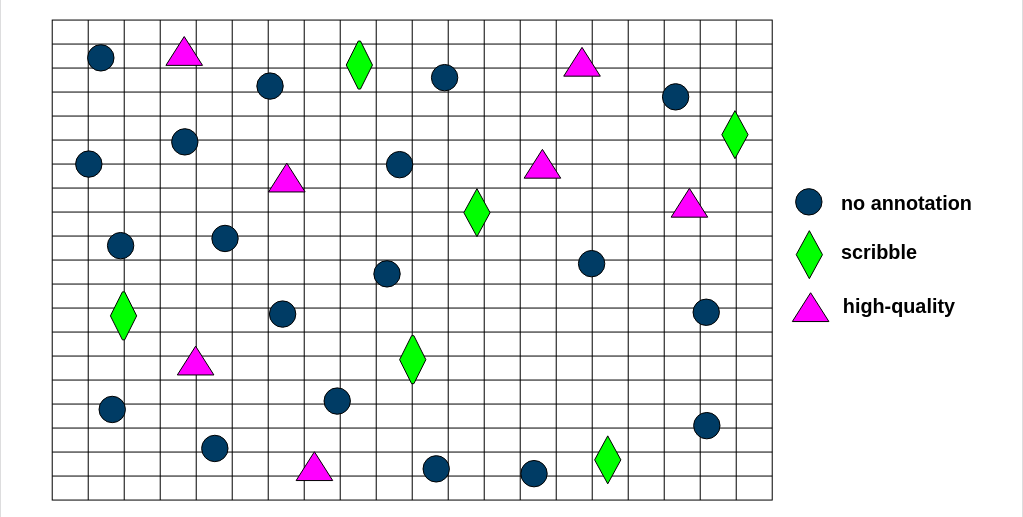
\includegraphics[width=0.85\linewidth]{images/figure_09}
	\end{figure}
\end{frame}


\begin{frame}{The problem}
	\begin{figure}
		\centering
		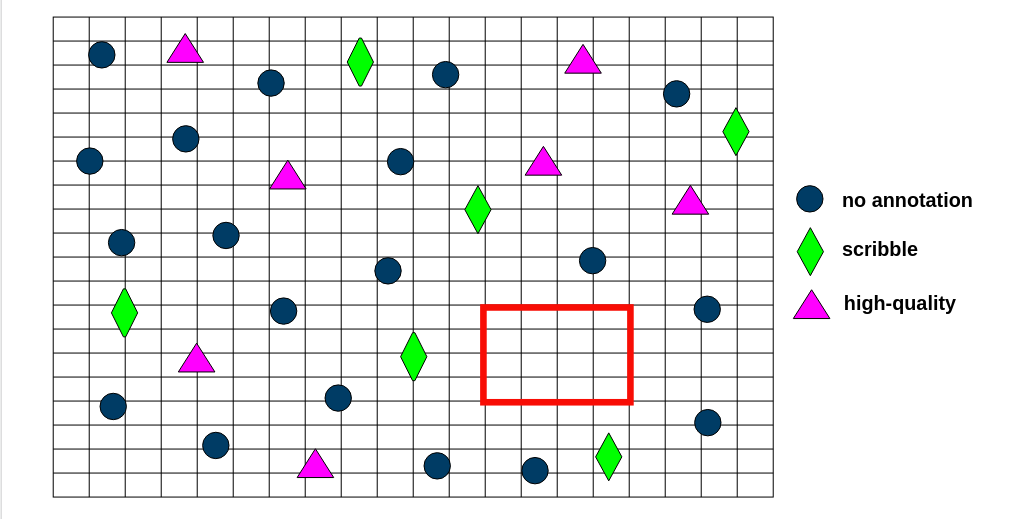
\includegraphics[width=0.85\linewidth]{images/figure_10}
	\end{figure}
\end{frame}


\begin{frame}{The problem}
	\begin{itemize}
		\item How do the models perform spatially?
		\item Is there a correlation between model performance and cloud cover?
		\item How do the models do in the summer compared to the winter?
		\item How do the models perform at cloud borders?
		\item How do techniques based on physics and machine learning approaches compare?
	\end{itemize}

\bigskip
\centering
\textbf{Can we build a model that answers all of these?}

\end{frame}


\begin{frame}[fragile]{Gaussian process}
\framesubtitle{``Gaussian process can do everything that NN do but better"}
Input and Output Data:
\begin{equation*}
\begin{array}{c}
	\mathbf{y}=\left(y_{1}, \ldots, y_{N}\right), \quad \mathbf{X}=\left(\mathbf{x}_{1}, \ldots, \mathbf{x}_{N}\right)^{\top} \\\\
	p(\mathbf{y} \mid \mathbf{f})=\mathcal{N}\left(\mathbf{y} \mid \mathbf{f}, \sigma^{2} \mathbf{I}\right), \quad p(\mathbf{f} \mid \mathbf{X})=\mathcal{N}(\mathbf{f} \mid 0, \mathbf{K}(\mathbf{X}, \mathbf{X}))
\end{array}
\end{equation*}

\begin{figure}
	\centering
	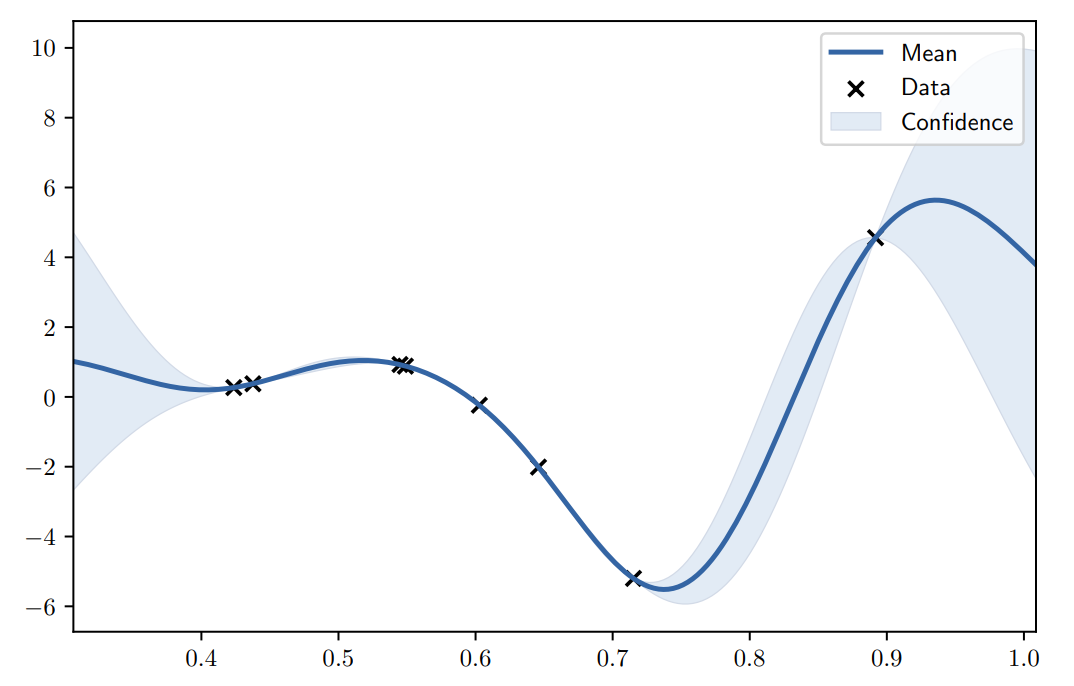
\includegraphics[width=0.5\linewidth]{images/figure_11}
	\label{fig:figure11}
\end{figure}
\end{frame}



\begin{frame}[fragile]{Gaussian process}
\begin{itemize}
\item Maximum likelihood estimate of the hyper-parameters.
$$
\theta^{*}=\underset{\theta}{\arg \max } \log p(\mathbf{y} \mid \mathbf{X}, \theta)=\underset{\theta}{\arg \max } \log \mathcal{N}\left(\mathbf{y} \mid 0, \mathbf{K}+\sigma^{2} \mathbf{I}\right)
$$
\item Prediction on a test point given the observed data and the optimized hyper-parameters.
$$
\begin{aligned}
	p\left(\mathbf{f}_{*} \mid \mathbf{X}_{*}, \mathbf{y}, \mathbf{X}, \theta\right)= &
	\mathcal{N}\left(\mathbf{f}_{*} \mid \mathbf{K}_{*}\left(\mathbf{K}+\sigma^{2} \mathbf{I}\right)^{-1} \mathbf{y}, \mathbf{K}_{* *}-\mathbf{K}_{*}\left(\mathbf{K}+\sigma^{2} \mathbf{I}\right)^{-1} \mathbf{K}_{*}^{\top}\right)
\end{aligned}
$$		
\end{itemize}
\end{frame}



\begin{frame}[fragile]{Gaussian process}

\begin{itemize}
\item Plug in the log-pdf of multi-variate normal distribution:
$$
\begin{aligned}
	\log p(\mathbf{y} \mid \mathbf{X}) &=\log \mathcal{N}\left(\mathbf{y} \mid 0, \mathbf{K}+\sigma^{2} \mathbf{I}\right) \\
	&=-\frac{1}{2} \log \left|2 \pi\left(\mathbf{K}+\sigma^{2} \mathbf{I}\right)\right|-\frac{1}{2} \mathbf{y}^{\top}\left(\mathbf{K}+\sigma^{2} \mathbf{I}\right)^{-1} \mathbf{y} \\
	&=-\frac{1}{2}\left(\left\|\mathbf{L}^{-1} \mathbf{y}\right\|^{2}+N \log 2 \pi\right)-\sum_{i} \log \mathbf{L}_{i i}
\end{aligned}
$$
\item Take a Cholesky decomposition: $\mathbf{L}=\operatorname{chol}\left(\mathbf{K}+\sigma^{2} \mathbf{I}\right)$.
\item The computational complexity is \textbf{$O\left(N^{3}+N^{2}+N\right)$}. Therefore, the overall complexity including the computation of $\mathbf{K}$ is $O\left(N^{3}\right)$.
\end{itemize}
\end{frame}

\begin{frame}{Gaussian process}
\begin{itemize}
	\item I collect the run time for $N = {10, 100, 500, 1000, 1500, 2000}$.
	\item They take $1.3ms, 8.5ms, 28ms, 0.12s, 0.29s, 0.76s$.

	\begin{figure}
		\centering
		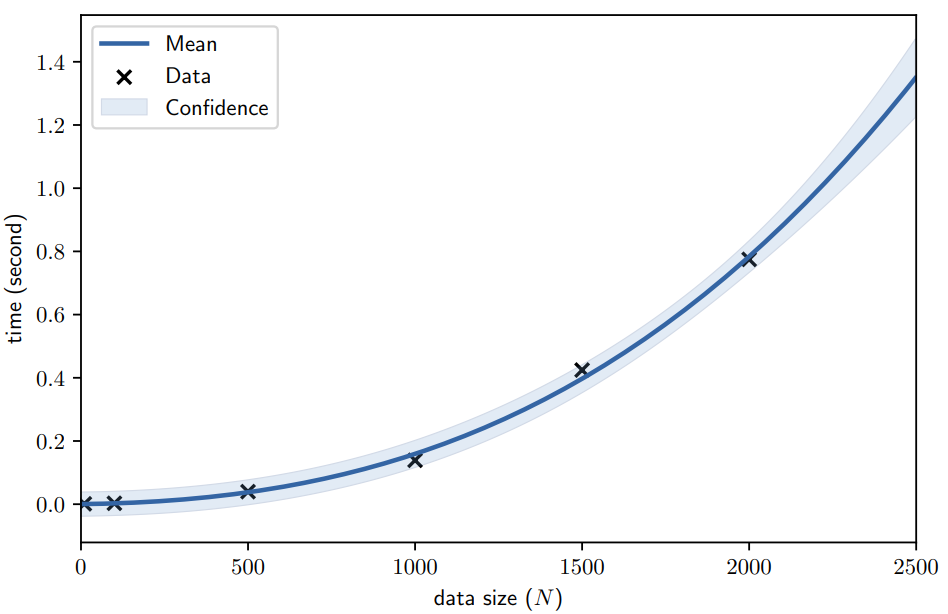
\includegraphics[width=0.5\linewidth]{images/figure_12}
		\label{fig:figure11}
	\end{figure}

	\item For 18000 points estimate the hyper-parameters will take approximately 27 hours.
\end{itemize}	
\end{frame}

\begin{frame}{Gaussian process}
	With redundant data, the covariance matrix becomes low rank.	
	\begin{columns}
		\begin{column}{0.5\textwidth}
			\begin{figure}
				\centering
				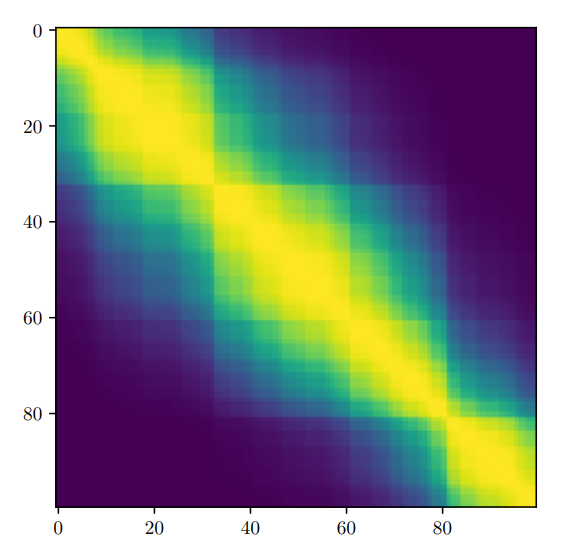
\includegraphics[width=0.8\linewidth]{images/figure_13}
				\label{fig:figure11}
			\end{figure}	
		\end{column}
		\begin{column}{0.5\textwidth}
			\begin{itemize}[<+->]
				\item Low rank Gaussian Process.
				\item Sparse Gaussian Process.
			\end{itemize}
		\end{column}
\end{columns}
\end{frame}


\begin{frame}{Scalable Gaussian process}
	\begin{itemize}
		\item BlackBox Matrix-Matrix Inference (BBMM).				
		\item LancZos Variance Estimates (LOVE).
		\bigskip	
		\begin{figure}
			\centering
			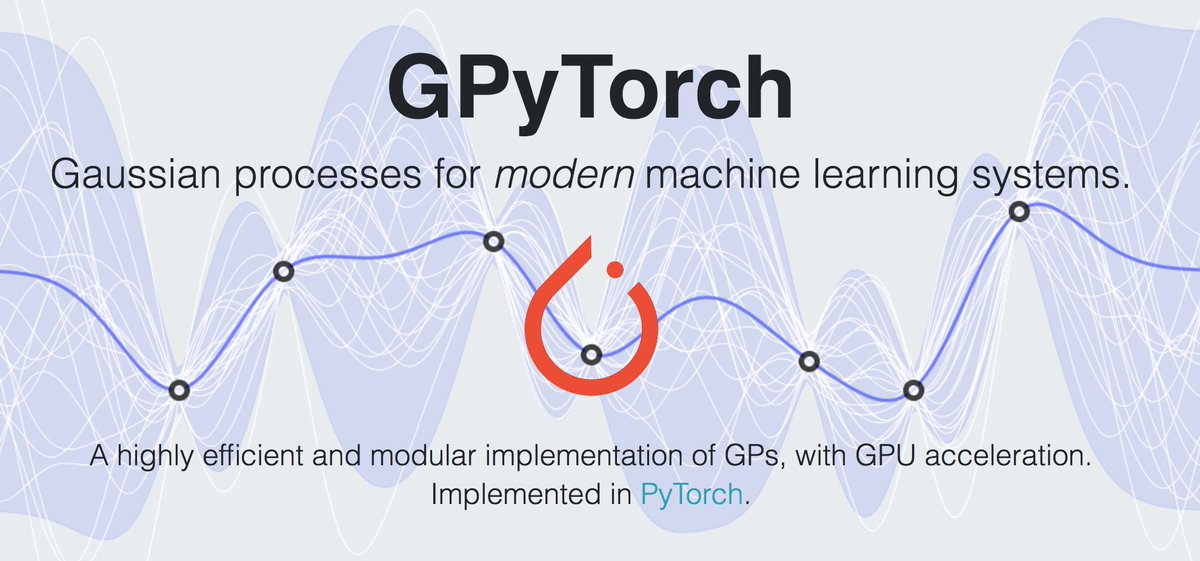
\includegraphics[width=0.6\linewidth]{images/figure_14}
			\label{fig:figure11}
		\end{figure}
	\end{itemize}
	\centering
	\textbf{\hrefcol{https://gpytorch.ai/}{https://gpytorch.ai/}}
\end{frame}



\begin{frame}{Geographically Weighted Gaussian Process}	
\begin{itemize}
	\item \textbf{Inputs} : Points distributed around the world $(X, Y, M)$.
	\item \textbf{Output} : Predicted values of regression points.
	\item \textbf{Variables:} 
	\begin{itemize}
		\item \textbf{bw:} Geographically Bandwidth.
		\item \textbf{Kn:} Kernel function.
		\item \textbf{Ln:} Linear Regression parameters.
		\item \textbf{Cn:} Covariance matrix.
	\end{itemize}
\end{itemize}
\end{frame}

\begin{frame}[fragile]{Nonstationary Gaussian Process}
\begin{block}{Locally Weighted Gaussian Process Approach}
	\begin{verbatim}
		for each updated sets of reference points Rfp do:
			- Create X and Y matrices.
			for i = 1 to number of regression points Rn do:				
				- Calculate W neighborhood matrix using bw, Kn and the distance between reference points Rfp and point i.
				- Calculate the regression coefficients (β): β(i) = (XTW(i)X)−1XTW(i)Y
				- Estimate the predicted value of yhat for point i using
				β(i) and Xi (a row vector).
				- Obtain the residuals comparing y vs yhat.
				- Use a GP to spatially the residuals.
				- Sum yhat with the residuals to get the final values.							
	\end{verbatim}
\end{block}
\end{frame}


\begin{frame}[fragile]{MixedKernel:}

The coordinates in our model is set as:

$$(x, y , M)$$

Using Hamming distances we created a combined kernel:

$$
K((x1, c1), (x2, c2)) = Kcont1(x1, x2) + Kcat1(c1, c2) + Kcont2(x1, x2) * Kcat2(c1, c2)
$$

where $xi$ and $ci$ are the continuous and categorical features of the
input, respectively. The suffix $i$ indicates that we fit different
lengthscales for the kernels in the sum and product terms.

\end{frame}



\begin{frame}[fragile]{TODO:}
	\begin{itemize}[<+->]
		\item Can the Gaussian Process predict the weights of the local linear model?
		\item Try to use a non-linear model (NN) to predict the weights.
		\item The idea is solve the following questions:
			\begin{itemize}
				\item \textbf{How do the models perform spatially?:} Train a GP using the entire dataset.
				\item \textbf{How do the models do in the summer compared to the winter?}: Train a GP splitting first the data by season.
				\item \textbf{How do the models perform at cloud borders?:} Train a GP using just information at borders.
				\item \textbf{How do techniques based on physics and machine learning approaches compare?:} Compare results between models.
			\end{itemize}
		\item Using GP and a DL models pretrained in cloudSEN12 we can predict the areas that need more annotations!.
		\item Considering the variance information we can propose a joined algorithm: $$dilation(X1*sen2cor + X2*s2cloudless + X3*QA)$$.
		\item \textbf{This would be the first cloud detection algorithm geographically aware!}
	\end{itemize}
\end{frame}


\begin{frame}[fragile]{Next steps:}
	\begin{itemize}
		\item Finish to write the chapter one (cloudSEN12 description).
		\item Create predictors: $X$
		\item Create a tabular dataset with the columns: $x, y, M, cc (target)$.
		\item Implement the algorithm described above.
		\item Create a $GP$ model for each question.
		\item Write chapter two.
	\end{itemize}
\end{frame}



\end{document}
